%%%%%%%%%%%%%%%%%%%%%%%%%%%%%%%%%%%%%%%%%%%%%%%%%%%%%%%%%%%%%%%%%%%%%%%%%%%%%%%%
\chapter{Экспериментальные данные (DREAM)}
\label{chapt2}

Проект DREAM предоставляет унифицированные экспериментальные данные для 
тестирования алгоритмов. Каждое «испытание» — некая формализованная задача,
которую предлагается решить независимым группам исследователей. Лучшие 
решения в результате публикуются \cite{bib6}. 

В рамках этой работы требуется подобрать близкие к оптимальным значения 
параметров ППРЭ, используя в качестве тестовых задач результаты DREAM6.

%%%%%%%%%%%%%%%%%%%%%%%%%%%%%%%%%%%%%%%%%%%%%%%%%%%%%%%%%%%%%%%%%%%%%%%%%%%%%%%%
\section{Постановка задачи} \label{sect2_1}

Эта задача принадлежит области обратной инженерии генно-регуляторных сетей. 
Предполагается, что топология генной сети уже определена с достаточным уровнем 
правдоподобия, и теперь требуется охарактеризовать параметры (кинетику) 
этой сети.

Здесь есть два ключевых аспекта, которые требуют внимания: задача оценки 
параметров модели по данной структуре модели, а так же задача проектирования 
наиболее информативных экспериментов для получения неизвестных параметров. 

Итак, даны структуры трёх генно-регуляторных сетей, от участников требуется 
разработать и/или применять методы оптимизации, чтобы точно оценить 
параметры моделей а так же прогнозировать результаты возмущений в этих моделях.

Эти две задачи и являются областью исследования DREAM6. Однако, для тестирования
ППРЭ потребуется рассмотреть лишь первую задачу.

%%%%%%%%%%%%%%%%%%%%%%%%%%%%%%%%%%%%%%%%%%%%%%%%%%%%%%%%%%%%%%%%%%%%%%%%%%%%%%%%
\section{Описание моделей генных сетей} \label{sect2_2}

Полные структуры генных сетей представлены в формате sbml, tic, и в графическом 
формате. Пример такого представления для первой генной сети приведён на 
рисунке~\ref{img:GrnImage}.

\begin{figure}[h]
  \center{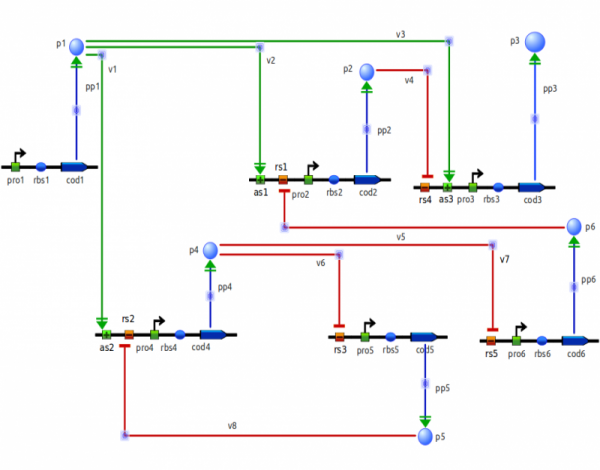
\includegraphics[width=14cm]{model1-600x470.png}}
  \caption{Пример графического представления для первой генной сети}
  \label{img:GrnImage}
\end{figure}

\begin{figure}[h]
  \center{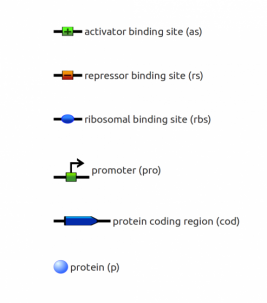
\includegraphics[width=7cm]{diagram_key-267x303.png}}
  \caption{Аннотация к графическому представлению}
  \label{img:GrnImageDesc}
\end{figure}

Для каждой сети предоставляется файл (.m) с описанием модели в 
синтаксисе MATLAB. Все переменные помечены в соответствии с их типом. 
Например, переменные, означабщие концентрацию белка, помечены как 
$p1$,~$p2$,~...~$p6$. 

Значения каждого символа в генной сети подробно 
объясняются в легенде (рис.~\ref{img:GrnImageDesc}). В скобках перечислены 
префиксы к переменным модели. Линии, соединяющие кодирующую белок 
последовательность с белком, обозначены префиксом «pp». Генерация белка состоит 
из двух логических частей: транскрипция и трансляция. Для простоты, эти два 
этапа, изображённые на схеме~\ref{img:GrnImageTT}, не показаны в диаграмме 
генной сети. 

Имена переменных для мРНК, для результата транскрипции кодирующей 
последовательности, так же имеют соответствующий префикс «pp». Например, мРНК, 
соответствующая $pp3$ будет именована как $pp3\_mrna$.

\begin{figure}[h]
  \center{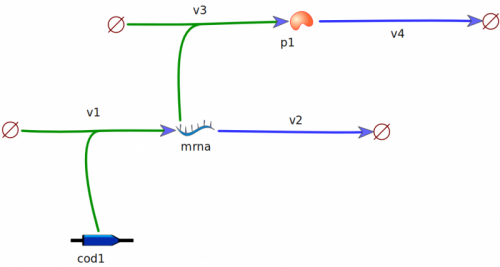
\includegraphics[width=12cm]{protein_production_subfigure-500x267.png}}
  \caption{Транскрипция и трансляция, не показаные на схеме генной сети}
  \label{img:GrnImageTT}
\end{figure}

%%%%%%%%%%%%%%%%%%%%%%%%%%%%%%%%%%%%%%%%%%%%%%%%%%%%%%%%%%%%%%%%%%%%%%%%%%%%%%%%
